
\section*{Question 3}

\begin{enumerate}[(a)]
    \item
    N=840\\
    \begin{figure}[h]
        \centering
        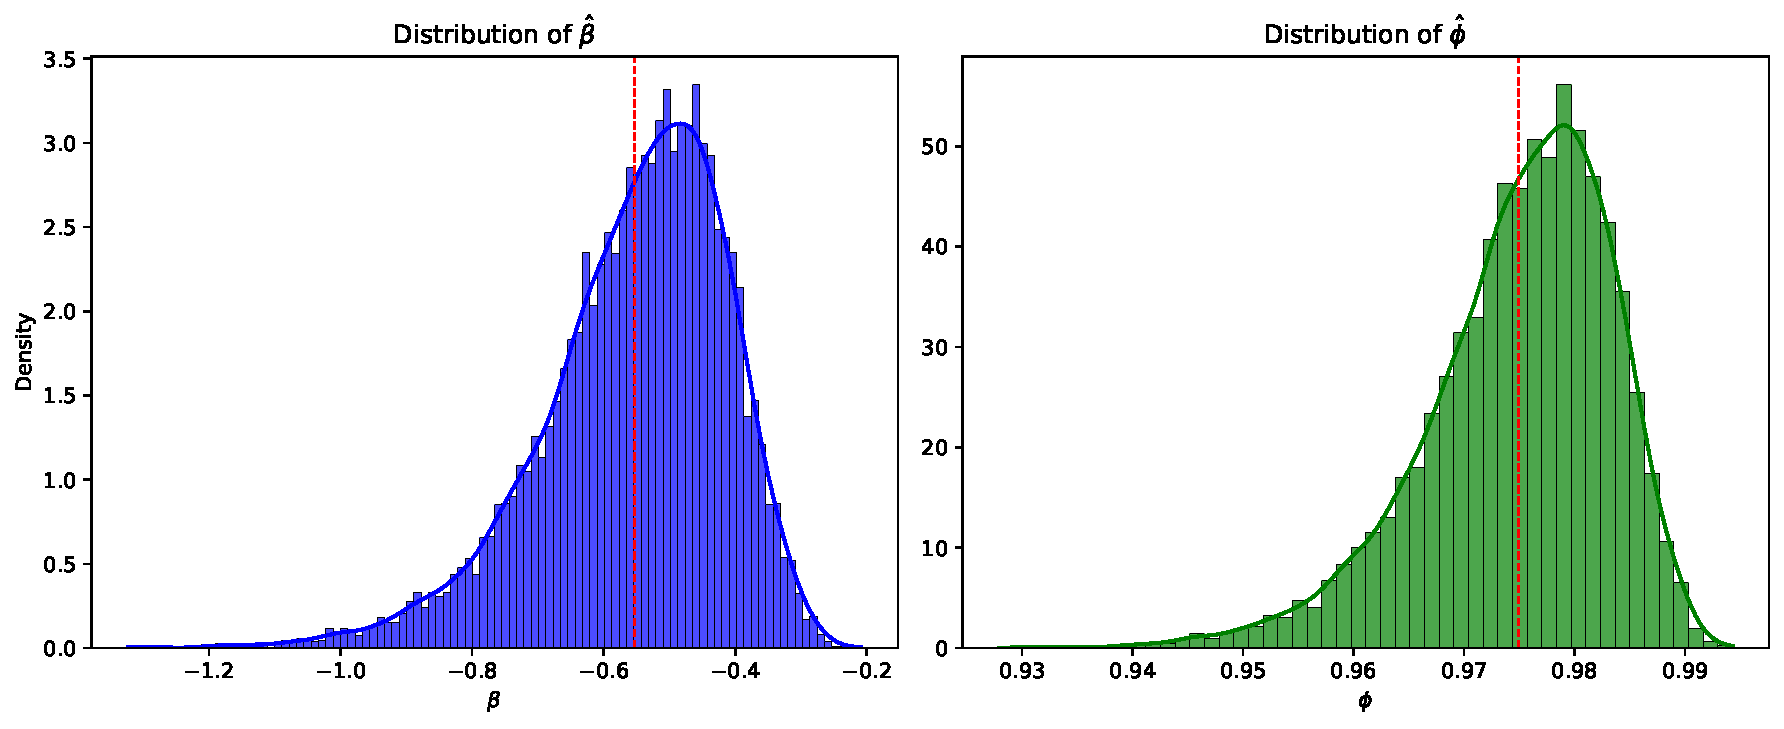
\includegraphics[width=0.9\linewidth]{Out/EX3-1.pdf}
        
    \end{figure}

  \item
    N=240\\
    \begin{figure}[h]
        \centering
        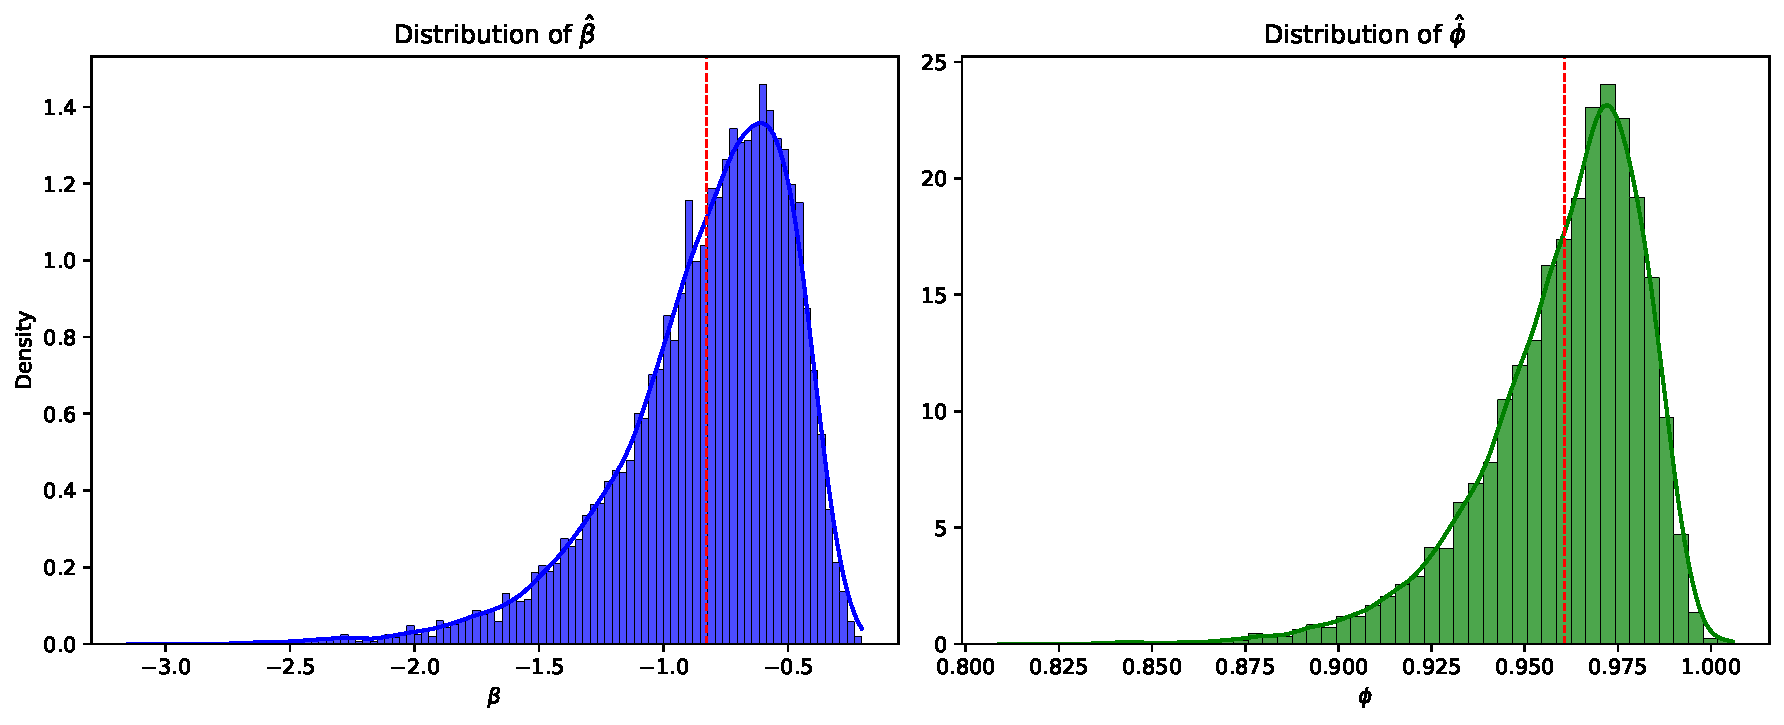
\includegraphics[width=0.9\linewidth]{Out/EX3-2.pdf}
        
    \end{figure}
Looks more skewed to the right side for $\hat{\phi}$
\item 
A rejection rate of 475 out of 10,000 replications corresponds to a 4.75\% rejection rate. In hypothesis testing, this would be close to the commonly chosen significance level of 5\%. The reason for this difference might be that the number of replications is not big enough and we need to conduct more simulations to see a more precise result; however, 4.75\% is quite close to the ideal 5\% level.

\item 
The null hypothesis (H0) is rejected 512 times out of 10,000 when using Newey-West standard errors, suggesting that there might be autocorrelation present in the errors, and the standard errors are adjusted to account for this.\\

Comparing this result to the rejection rate from problem 3b (475 out of 10,000) when standard errors assuming IID errors were used, the increased number of rejections and being closer to the 5\% ideal level with Newey-West standard errors indicate that autocorrelation might be influencing the precision of the coefficient estimates.
\end{enumerate}
